\documentclass[border=6pt]{standalone}
% Shared preamble for web figures.  Each figure is a standalone .tex that
% \input's this file; scripts/make-figures.sh turns it into an SVG.
% Handouts pull the same file with \fig{Unit_X/<name>}.
\usepackage[T1]{fontenc}
\usepackage{helvet}
\renewcommand{\familydefault}{\sfdefault}
\usepackage{amsmath}
\usepackage{tikz}
\usetikzlibrary{arrows.meta,positioning,calc,shapes.symbols,shapes.geometric}

% Who makes the rules is the point of most diagrams in this book, so the
% colors mean the same thing everywhere: blue is a person, orange is the
% computer, green is an answer, pink is the human brain.
\definecolor{person}{HTML}{2C6FAE}
\definecolor{machine}{HTML}{D35400}
\definecolor{result}{HTML}{1E8449}
\definecolor{brainpink}{HTML}{C2185B}
\definecolor{ink}{HTML}{2C3E50}

\tikzset{
  doodle/.style={line width=1.5pt, line cap=round, line join=round, draw=ink},
  box/.style={draw, rounded corners=5pt, line width=1.1pt, align=center,
              inner sep=7pt, minimum height=1.0cm, font=\small},
  personbox/.style={box, draw=person, fill=person!10},
  machinebox/.style={box, draw=machine, fill=machine!10},
  resultbox/.style={box, draw=result, fill=result!10},
  plainbox/.style={box, draw=ink!70, fill=ink!4},
  flow/.style={-{Stealth[length=8pt]}, line width=1.4pt, draw=ink},
}

\begin{document}
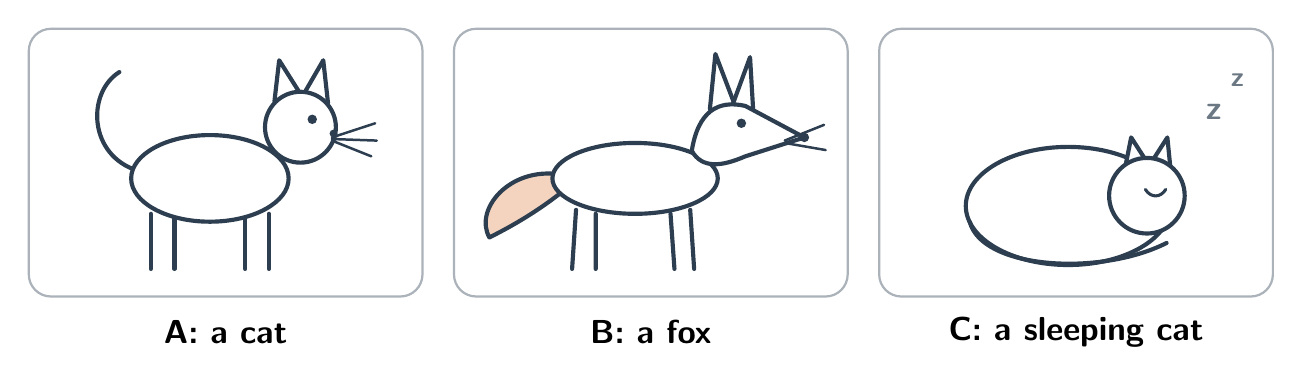
\begin{tikzpicture}
% Three doodles to test a student's rule for "cat".  A passes, B (a fox)
% passes when it should not, C (a cat curled up) fails when it should pass.

% ---------- A: a cat ----------
\begin{scope}
  \draw[rounded corners=8pt, ink!40, line width=0.8pt] (-0.4,0) rectangle (4.6,3.4);
  \draw[doodle] (1.15,1.05) -- (1.15,0.35) (1.45,1.0) -- (1.45,0.35)
                (2.35,1.0) -- (2.35,0.35) (2.65,1.05) -- (2.65,0.35);
  \draw[doodle, fill=white] (1.9,1.5) ellipse (1.0 and 0.55);
  \draw[doodle] (0.92,1.62) .. controls (0.35,1.85) and (0.35,2.6) .. (0.75,2.85);
  \draw[doodle, fill=white] (2.72,2.48) -- (2.78,3.0) -- (3.02,2.62);
  \draw[doodle, fill=white] (3.12,2.62) -- (3.34,3.0) -- (3.40,2.46);
  \draw[doodle, fill=white] (3.05,2.15) circle (0.45);
  \fill[ink] (3.2,2.25) circle (0.06);
  \fill[ink] (3.47,2.07) circle (0.05);
  \draw[doodle, line width=0.9pt] (3.45,2.02) -- (4.0,2.2) (3.45,2.0) -- (4.02,1.98) (3.45,1.98) -- (3.95,1.78);
  \node[font=\large\bfseries] at (2.1,-0.45) {A: a cat};
\end{scope}

% ---------- B: a fox ----------
\begin{scope}[xshift=5.4cm]
  \draw[rounded corners=8pt, ink!40, line width=0.8pt] (-0.4,0) rectangle (4.6,3.4);
  \draw[doodle] (1.15,1.1) -- (1.1,0.35) (1.4,1.05) -- (1.4,0.35)
                (2.35,1.05) -- (2.4,0.35) (2.6,1.1) -- (2.65,0.35);
  % bushy tail with a white tip
  \draw[doodle, fill=machine!25] (0.95,1.55) .. controls (0.3,1.65) and (-0.15,1.1) .. (0.05,0.75)
        .. controls (0.45,0.95) and (0.75,1.15) .. (1.0,1.35);
  \draw[doodle, fill=white] (1.9,1.5) ellipse (1.05 and 0.45);
  \draw[doodle, fill=white] (2.85,2.38) -- (2.92,3.08) -- (3.16,2.45);
  \draw[doodle, fill=white] (3.14,2.44) -- (3.36,3.04) -- (3.40,2.36);
  \draw[doodle, fill=white] (2.62,1.85) .. controls (2.7,2.35) and (2.95,2.5) .. (3.3,2.42)
        -- (4.05,2.02) -- (3.3,1.78) .. controls (3.0,1.65) and (2.75,1.62) .. cycle;
  \fill[ink] (3.25,2.2) circle (0.06);
  \fill[ink] (4.05,2.02) circle (0.06);
  \draw[doodle, line width=0.9pt] (3.8,1.98) -- (4.3,2.18) (3.8,1.95) -- (4.32,1.86);
  \node[font=\large\bfseries] at (2.1,-0.45) {B: a fox};
\end{scope}

% ---------- C: a cat curled up asleep ----------
\begin{scope}[xshift=10.8cm]
  \draw[rounded corners=8pt, ink!40, line width=0.8pt] (-0.4,0) rectangle (4.6,3.4);
  \draw[doodle, fill=white] (2.0,1.15) ellipse (1.3 and 0.75);
  \draw[doodle, fill=white] (2.72,1.62) -- (2.80,2.02) -- (2.98,1.74);
  \draw[doodle, fill=white] (3.08,1.74) -- (3.26,2.02) -- (3.30,1.62);
  \draw[doodle, fill=white] (3.0,1.28) circle (0.48);
  \draw[doodle, line width=1.1pt] (2.98,1.36) .. controls (3.05,1.25) and (3.17,1.25) .. (3.24,1.36);
  \draw[doodle] (0.75,0.95) .. controls (0.9,0.35) and (2.4,0.25) .. (3.25,0.68);
  \node[font=\bfseries\large, ink!70] at (3.85,2.35) {z};
  \node[font=\bfseries, ink!70] at (4.15,2.75) {z};
  \node[font=\large\bfseries] at (2.1,-0.45) {C: a sleeping cat};
\end{scope}
\end{tikzpicture}
\end{document}
